% Drawing 154/01-3 -- folder 154, batch 01, archive page 3 (PDF page 4).
% Transcription: figure : $\mathcal{X}'_1$ pour $n = 5$ --- un petit disque au bord pointillé de rouge, traversé par un arrangement de pseudo-droites rouges, d'où rayonnent en alternance des traits rouges et jaunes
% Kind: pseudoline arrangement in a disk with rays (X'_1). Method 2 (schematic redraw from the facsimile). Status: partial.
% Notes: A small disk with a red dotted rim crossed by a few red pseudolines, from which red and yellow strokes radiate alternately (about 28 rays, the count approximate); legend X'_1 pour n = 5. The inner strands are schematic. Still differs from the facsimile: A small disk with a red dotted rim crossed by a few red pseudolines, from which red and yellow strokes radiate alternately (about 28 rays, the count approximate); legend X'_1 pour n = 5. The inner strands are schematic.
% Coordinates: 1 unit = 1 mm = 1/100 of the crop width (bbox in page fractions: [0.618, 0.108, 0.939, 0.263]).
% Redrawn by Claude (claude-opus-5-5), issue #73, 2026-11-07; not checked by a human; not compiled (no TeX in the session).
% Revised by Claude (claude-opus-5-5) 2026-11-09 (issue #128) after Michel's check: vertices snapped to exact intersections (drawn points on their lines, meeting ends on the stroke they meet, near-concurrent lines through one computed point, curve ends on their rim); labels at \small as in folder 80 batch 3. Status: partial.
% Rights: reproduces part of the work -- behind RENDER_TRANSCRIPTS, never published by itself.
\documentclass[tikz,border=3pt]{standalone}
\usepackage{amsmath,amssymb}
\usetikzlibrary{patterns,arrows.meta}
\tikzset{Or/.style={orange!90!black}, Ye/.style={yellow!80!orange}, Lg/.style={green!60!black!70}, Dg/.style={green!45!black}, Br/.style={brown!80!black}, Rd/.style={red!85!black}, Bl/.style={blue!70!black}, Gy/.style={black!40}, pencil/.style={black!45}, struck/.style={black!35}, mark/.style={circle,draw,inner sep=1.3pt}, pt/.style={circle,fill,inner sep=0.9pt}, opt/.style={circle,draw,fill=white,inner sep=1.1pt}}
\begin{document}
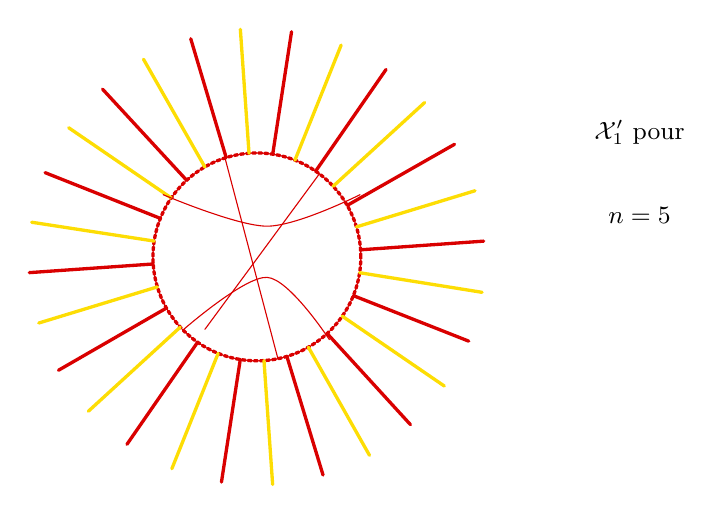
\begin{tikzpicture}[x=1mm,y=1mm,line cap=round,line join=round,font=\scriptsize]
\draw[Rd,densely dotted,very thick] (38.2,-34.2) circle[radius=13.2];
\draw[Rd,very thick] (51.37,-33.3) -- (67,-32.2);
\draw[Ye,very thick] (50.84,-30.39) -- (65.9,-25.8);
\draw[Rd,very thick] (49.67,-27.66) -- (63.3,-19.9);
\draw[Ye,very thick] (47.88,-25.23) -- (59.5,-14.6);
\draw[Rd,very thick] (45.66,-23.31) -- (54.6,-10.4);
\draw[Ye,very thick] (43.03,-21.92) -- (48.9,-7.3);
\draw[Rd,very thick] (40.21,-21.15) -- (42.6,-5.6);
\draw[Ye,very thick] (37.2,-21.04) -- (36.1,-5.3);
\draw[Rd,very thick] (34.3,-21.59) -- (29.8,-6.5);
\draw[Ye,very thick] (31.59,-22.78) -- (23.8,-9.1);
\draw[Rd,very thick] (29.28,-24.47) -- (18.6,-12.9);
\draw[Ye,very thick] (27.33,-26.72) -- (14.3,-17.8);
\draw[Rd,very thick] (25.94,-29.31) -- (11.3,-23.5);
\draw[Ye,very thick] (25.15,-32.19) -- (9.6,-29.8);
\draw[Rd,very thick] (25.03,-35.1) -- (9.3,-36.2);
\draw[Ye,very thick] (25.56,-38.01) -- (10.5,-42.6);
\draw[Rd,very thick] (26.71,-40.7) -- (13,-48.6);
\draw[Ye,very thick] (28.47,-43.12) -- (16.8,-53.8);
\draw[Rd,very thick] (30.67,-45.04) -- (21.7,-58);
\draw[Ye,very thick] (33.28,-46.45) -- (27.4,-61.1);
\draw[Rd,very thick] (36.09,-47.23) -- (33.7,-62.8);
\draw[Ye,very thick] (39.1,-47.37) -- (40.2,-63.1);
\draw[Rd,very thick] (42.01,-46.84) -- (46.6,-61.9);
\draw[Ye,very thick] (44.74,-45.67) -- (52.5,-59.4);
\draw[Rd,very thick] (47.12,-43.93) -- (57.7,-55.5);
\draw[Ye,very thick] (49.04,-41.73) -- (62,-50.6);
\draw[Rd,very thick] (50.45,-39.12) -- (65.1,-44.9);
\draw[Ye,very thick] (51.25,-36.21) -- (66.8,-38.7);
\draw[Rd] plot[smooth, tension=0.55] coordinates {(26.3,-26.3) (39.5,-30.3) (51.3,-26.3)};
\draw[Rd] plot[smooth, tension=0.55] coordinates {(28.82,-43.48) (39.5,-36.8) (47.4,-44.7)};
\draw[Rd] (34.15,-21.64) -- (40.87,-47.13);
\draw[Rd] (46.14,-23.65) -- (31.6,-43.4);
\node[inner sep=1pt] at (86.8,-18.4) {\small $\mathcal{X}'_1$ pour};
\node[inner sep=1pt] at (86.8,-28.9) {\small $n=5$};
\end{tikzpicture}
\end{document}
